\begin{frame}
    \frametitle{Anexo: One-Class SVM}

    \begin{itemize}
        \item
        \footnotesize Hiperplano del clasificador para el grupo $G_{i}$
    \end{itemize}

    \begin{equation}
        \vec{w_{i}} \cdot \phi(\vec{x})
        \ - \
        \rho_{i}
        \ = \
        \sum_{j=1}^{\lvert G_{i} \rvert}
        \left(
            a_{ij} \, K_{i}(\vec{f_{ij}}, \vec{x})
        \right)
        \ - \
        \rho_{i}
        \ = \
        0
    \end{equation}

    \begin{itemize}
        \item
        \footnotesize Kernel Radial Basis Function (RBF)
    \end{itemize}

    \begin{equation}
        K(\vec{x_{1}}, \vec{x_{2}})
        \ = \
        \phi(\vec{x_{1}}) \cdot \phi(\vec{x_{2}})
        \ = \
        \exp(
            - \gamma \lVert \vec{x_{1}} - \vec{x_{2}} \lVert^2
        )
    \end{equation}
\end{frame}

\begin{frame}
    \frametitle{Anexo: One-Class SVM}

    \begin{itemize}
        \item
        \footnotesize Entrenamiento: problema de minimización para el grupo $G_{i}$
    \end{itemize}

    \begin{equation}
        \min_{
            \vec{w_{i}}
            \ , \
            \rho_{i}
            \ , \
            \xi_{i}
        }
        \
        \frac{1}{2} \lVert {\vec{w_{i}}} \rVert^2
        \ - \
        \rho_{i}
        \ + \
        \frac{1}{\nu_{i} \lvert G_{i} \rvert} \sum_{j=1}^{\lvert G_{i} \rvert} \xi_{ij}
    \end{equation}

    \begin{equation}
        \vec{w_{i}} \cdot \phi(\vec{f_{ij}}) \geqslant \rho_{i} - \xi_{ij}
        \ , \quad
        \xi_{ij} \geqslant 0
        \ , \quad
        \forall j = 1,2, \dots, \lvert G_{i} \rvert
    \end{equation}

    \begin{itemize}
        \item
        \footnotesize Entrenamiento: formulación dual de la optimización
    \end{itemize}

    \begin{equation}
        \min_{a_{i}}
        \
        \frac{1}{2} \ a_{i} \ S_{i} \ a_{i}^{T}
    \end{equation}

    \begin{equation}
        \sum_{j=1}^{\lvert G_{i} \rvert} a_{ij} \ = \ 1
        \ , \quad
        0 \leqslant a_{ij} \leqslant \frac{1}{\nu_{i} \lvert G_{i} \rvert}
        \
        \forall j = 1,2, \dots, \lvert G_{i} \rvert
    \end{equation}
\end{frame}

\begin{frame}
    \frametitle{Anexo: One-Class SVM}

    \begin{itemize}
        \item
        \footnotesize Detección: función de decisión del grupo $G_{i}$
    \end{itemize}

    \begin{equation}
        g_{i}(\vec{x})
        \ = \
        \begin{cases}
            \vec{w_{i}} \cdot \phi(\vec{x}) - \rho_{i} \ \geqslant \ 0  & +1 \\
            \text{caso contrario}                                       & -1
        \end{cases}
    \end{equation}

    \begin{equation}
        g_{i}(\vec{x})
        \ = \
        \begin{cases}
            \sum_{j=1}^{\lvert G_{i} \rvert}
            \left(
                a_{ij} \, K_{i}(\vec{f_{ij}}, \vec{x})
            \right)
            - \rho_{i} \ \geqslant \ 0  & +1 \\
            \text{caso contrario}       & -1
        \end{cases}
    \end{equation}
\end{frame}

\begin{frame}
    \frametitle{Anexo: Datos utilizados para las pruebas}

    \begin{itemize}
        \item
        \footnotesize Información sobre los 18 grupos de peticiones
    \end{itemize}

    \begin{center}
        \tiny
        \begin{tabularx}{\linewidth}{|C|c|ll|r|r|r|}
            \hline
            ID
            & \multicolumn{1}{c|}{\begin{tabular}[c]{@{}c@{}}Conjunto\\ de datos\\ CSIC\end{tabular}}
            & \multicolumn{2}{c|}{Método HTTP y URL}
            & \multicolumn{1}{c|}{\begin{tabular}[c]{@{}c@{}}Cant.\\ parám.\end{tabular}}
            & \multicolumn{1}{c|}{\begin{tabular}[c]{@{}c@{}}Peticiones\\ normales\end{tabular}}
            & \multicolumn{1}{c|}{\begin{tabular}[c]{@{}c@{}}Peticiones\\ anómalas\end{tabular}} \\
            \specialrule{1.5pt}{0}{0}
            c00 & 2010  & GET  & /tienda1/miembros/editar.jsp         & 13 &  \num{2000} &  \num{1362} \\ \hline
            c01 & 2010  & POST & /tienda1/miembros/editar.jsp         & 13 &  \num{2000} &  \num{1362} \\ \hline
            c02 & 2010  & GET  & /tienda1/publico/anadir.jsp          &  5 &  \num{2000} &  \num{1380} \\ \hline
            c03 & 2010  & POST & /tienda1/publico/anadir.jsp          &  5 &  \num{2000} &  \num{1380} \\ \hline
            c04 & 2010  & GET  & /tienda1/publico/autenticar.jsp      &  5 &  \num{2000} &  \num{1361} \\ \hline
            c05 & 2010  & POST & /tienda1/publico/autenticar.jsp      &  5 &  \num{2000} &  \num{1361} \\ \hline
            c06 & 2010  & GET  & /tienda1/publico/caracteristicas.jsp &  1 &  \num{2000} &   \num{954} \\ \hline
            c07 & 2010  & POST & /tienda1/publico/caracteristicas.jsp &  1 &  \num{2000} &   \num{954} \\ \hline
            c08 & 2010  & GET  & /tienda1/publico/entrar.jsp          &  1 &  \num{2000} &   \num{897} \\ \hline
            c09 & 2010  & POST & /tienda1/publico/entrar.jsp          &  1 &  \num{2000} &   \num{897} \\ \hline
            c10 & 2010  & GET  & /tienda1/publico/pagar.jsp           &  3 &  \num{2000} &  \num{1343} \\ \hline
            c11 & 2010  & POST & /tienda1/publico/pagar.jsp           &  3 &  \num{2000} &  \num{1343} \\ \hline
            c12 & 2010  & GET  & /tienda1/publico/registro.jsp        & 13 &  \num{2000} &  \num{1364} \\ \hline
            c13 & 2010  & POST & /tienda1/publico/registro.jsp        & 13 &  \num{2000} &  \num{1364} \\ \hline
            c14 & 2010  & GET  & /tienda1/publico/vaciar.jsp          &  1 &  \num{2000} &   \num{919} \\ \hline
            c15 & 2010  & POST & /tienda1/publico/vaciar.jsp          &  1 &  \num{2000} &   \num{919} \\ \hline
            t00 & 2012  & POST & /tienda1/miembros/editar.jsp         & 12 &  \num{5608} & \num{10121} \\ \hline
            t01 & 2012  & POST & /tienda1/publico/registro.jsp        & 12 &  \num{2522} & \num{13163} \\
            \specialrule{1.5pt}{0}{0}
                & Total &      &                                      &    & \num{40130} & \num{42444} \\ \hline
        \end{tabularx}
    \end{center}
\end{frame}

\begin{frame}
    \frametitle{Anexo: Resultados de detección}

    \begin{itemize}
        \item
        \footnotesize Resultados de los 18 grupos de peticiones
    \end{itemize}

    \begin{center}
        \tiny
        \begin{tabular}{|c|ccc|}
            \hline
            Grupo & TPR                         & FPR                         & $F_{1}$-\textit{score}      \\
            \specialrule{1.5pt}{0}{0}
            c00   & \num{0.71} $\pm$ \num{0.01} & \num{0.05} $\pm$ \num{0.00} & \num{0.80} $\pm$ \num{0.00} \\ \hline
            c01   & \num{0.72} $\pm$ \num{0.01} & \num{0.05} $\pm$ \num{0.01} & \num{0.80} $\pm$ \num{0.00} \\ \hline
            c02   & \num{1.00} $\pm$ \num{0.00} & \num{0.03} $\pm$ \num{0.01} & \num{0.98} $\pm$ \num{0.01} \\ \hline
            c03   & \num{1.00} $\pm$ \num{0.00} & \num{0.03} $\pm$ \num{0.00} & \num{0.98} $\pm$ \num{0.00} \\ \hline
            c04   & \num{0.91} $\pm$ \num{0.01} & \num{0.01} $\pm$ \num{0.00} & \num{0.95} $\pm$ \num{0.01} \\ \hline
            c05   & \num{0.92} $\pm$ \num{0.01} & \num{0.01} $\pm$ \num{0.00} & \num{0.95} $\pm$ \num{0.00} \\ \hline
            c06   & \num{0.99} $\pm$ \num{0.00} & \num{0.00} $\pm$ \num{0.00} & \num{1.00} $\pm$ \num{0.00} \\ \hline
            c07   & \num{0.99} $\pm$ \num{0.00} & \num{0.00} $\pm$ \num{0.00} & \num{1.00} $\pm$ \num{0.00} \\ \hline
            c08   & \num{1.00} $\pm$ \num{0.00} & \num{0.00} $\pm$ \num{0.00} & \num{1.00} $\pm$ \num{0.00} \\ \hline
            c09   & \num{1.00} $\pm$ \num{0.00} & \num{0.00} $\pm$ \num{0.00} & \num{1.00} $\pm$ \num{0.00} \\ \hline
            c10   & \num{1.00} $\pm$ \num{0.00} & \num{0.00} $\pm$ \num{0.00} & \num{1.00} $\pm$ \num{0.00} \\ \hline
            c11   & \num{1.00} $\pm$ \num{0.00} & \num{0.01} $\pm$ \num{0.00} & \num{0.99} $\pm$ \num{0.00} \\ \hline
            c12   & \num{0.74} $\pm$ \num{0.00} & \num{0.05} $\pm$ \num{0.01} & \num{0.81} $\pm$ \num{0.01} \\ \hline
            c13   & \num{0.74} $\pm$ \num{0.00} & \num{0.05} $\pm$ \num{0.01} & \num{0.81} $\pm$ \num{0.01} \\ \hline
            c14   & \num{1.00} $\pm$ \num{0.00} & \num{0.00} $\pm$ \num{0.00} & \num{1.00} $\pm$ \num{0.00} \\ \hline
            c15   & \num{1.00} $\pm$ \num{0.00} & \num{0.00} $\pm$ \num{0.00} & \num{1.00} $\pm$ \num{0.00} \\ \hline
            t00   & \num{0.99} $\pm$ \num{0.01} & \num{0.06} $\pm$ \num{0.04} & \num{0.98} $\pm$ \num{0.00} \\ \hline
            t01   & \num{1.00} $\pm$ \num{0.00} & \num{0.09} $\pm$ \num{0.06} & \num{0.99} $\pm$ \num{0.01} \\
            \specialrule{1.5pt}{0}{0}
                  & \num{0.93} $\pm$ \num{0.11} & \num{0.03} $\pm$ \num{0.03} & \num{0.95} $\pm$ \num{0.08} \\ \hline
        \end{tabular}
    \end{center}
\end{frame}

\begin{frame}
    \frametitle{Anexo: Resultados de detección}

    \begin{itemize}
        \item
        \footnotesize Resultados con anomalías entre los datos de entrenamiento
    \end{itemize}

    \begin{center}
        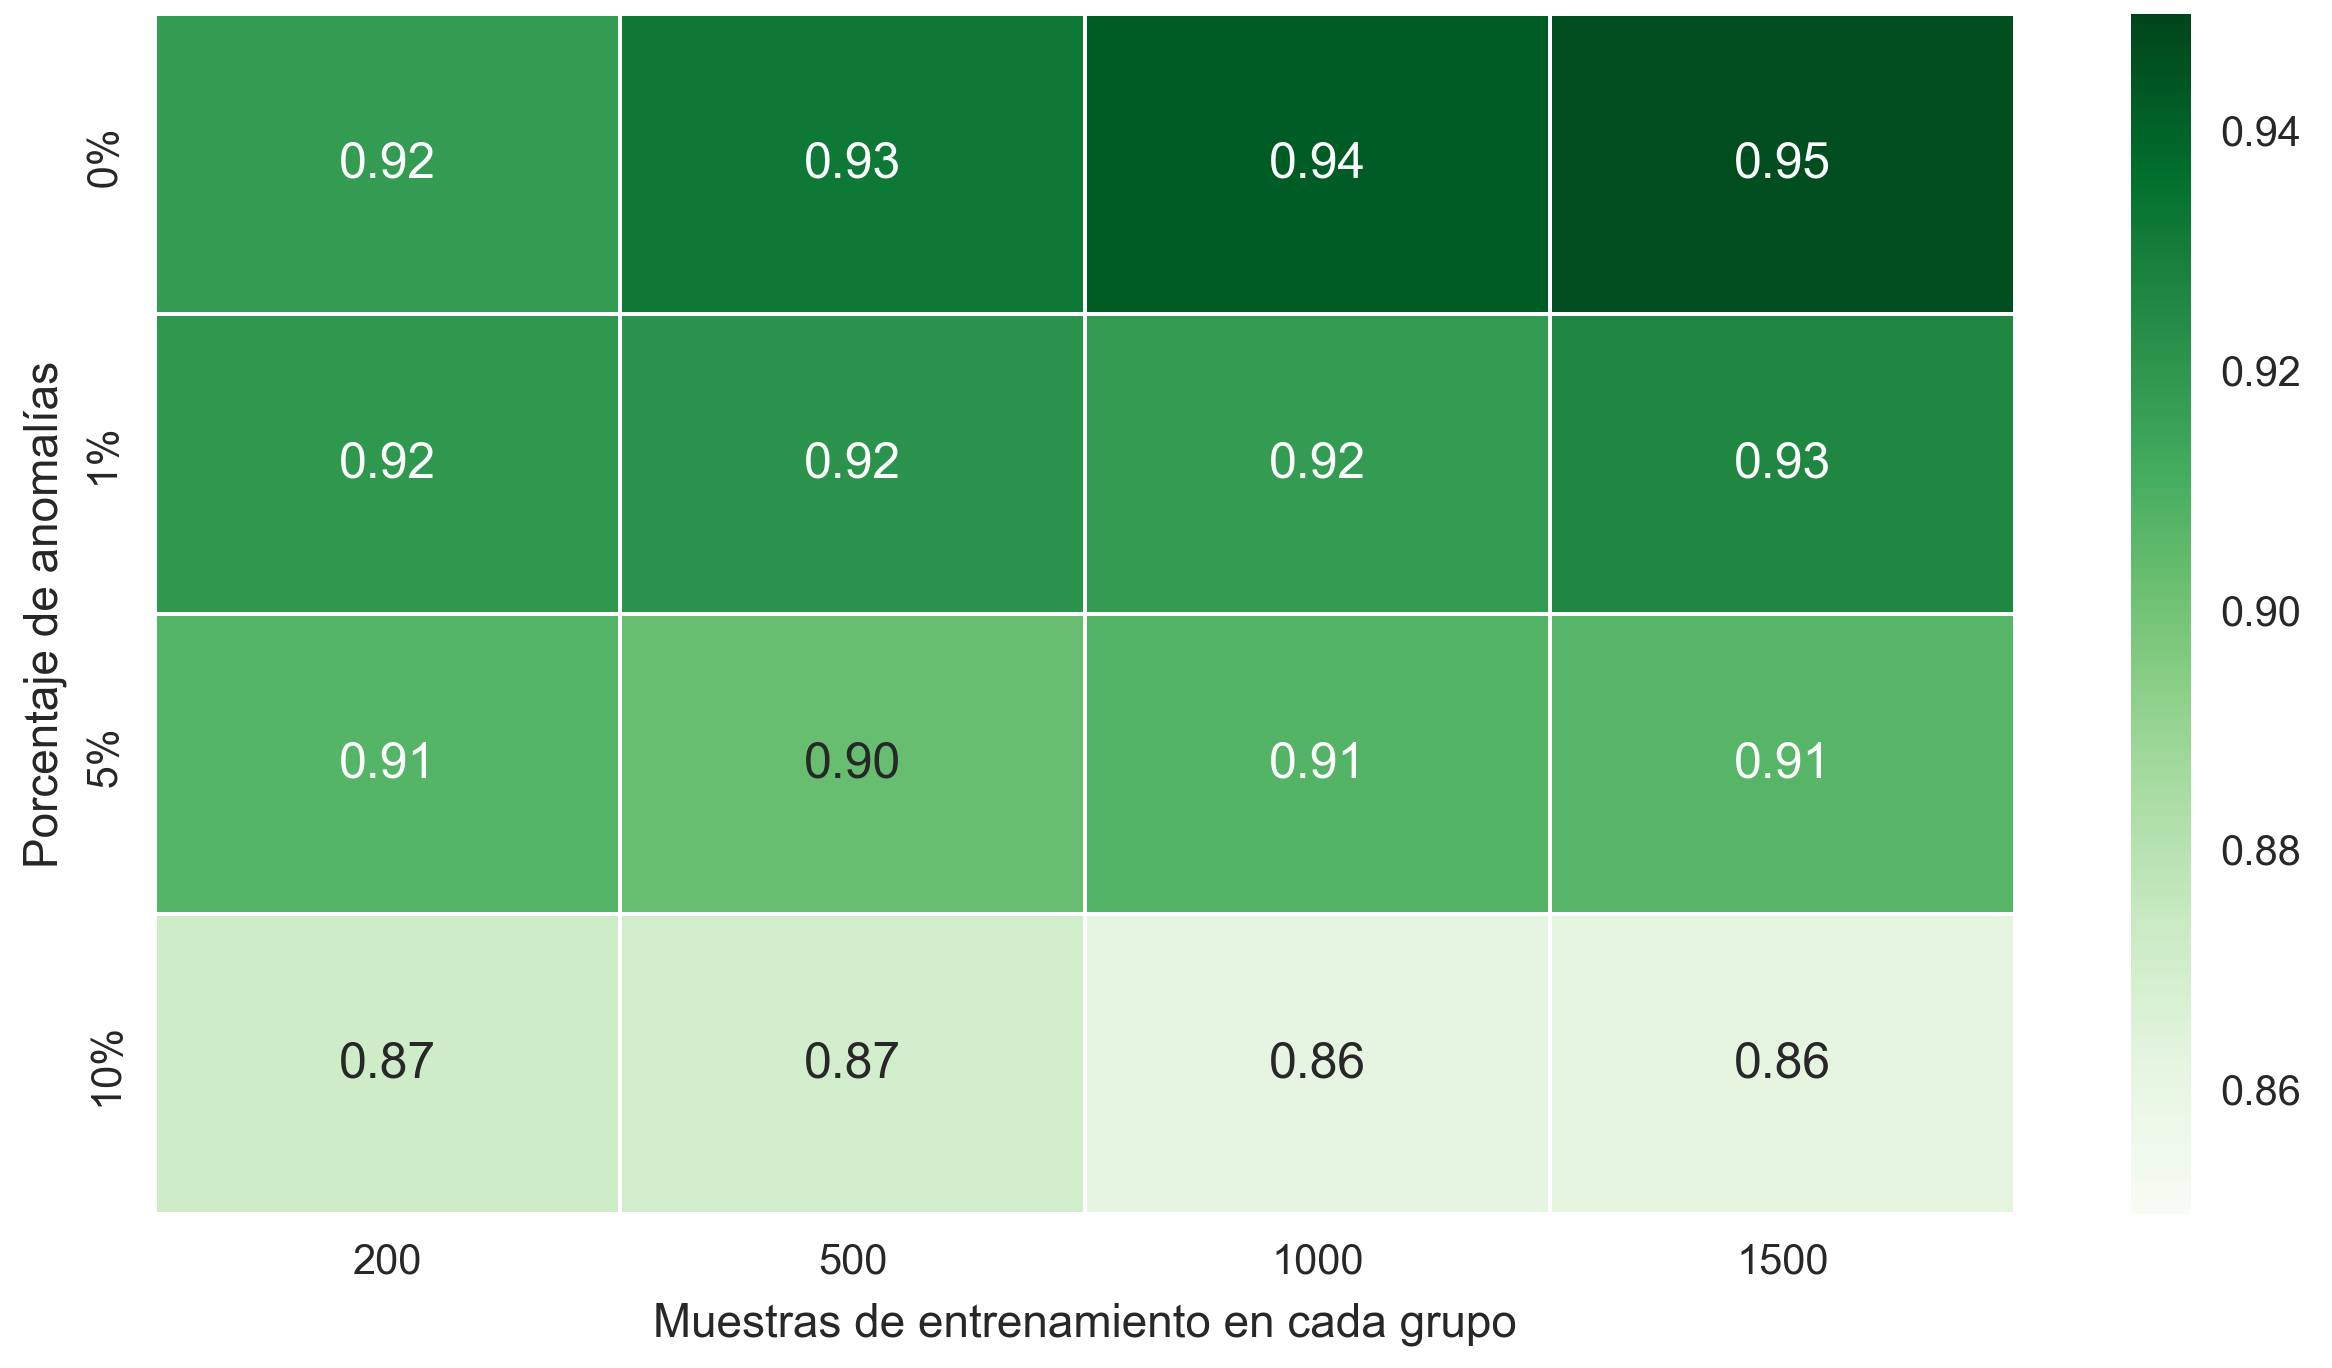
\includegraphics[width=\textwidth]{images/heatmap-results-training-anomalies.png}
    \end{center}
\end{frame}
